% !TEX TS-program = pdflatex
% !TEX encoding = UTF-8 Unicode

% This is a simple template for a LaTeX document using the "article" class.
% See "book", "report", "letter" for other types of document.

\documentclass[11pt]{article} % use larger type; default would be 10pt

\usepackage[utf8]{inputenc} % set input encoding (not needed with XeLaTeX)

%%% Examples of Article customizations
% These packages are optional, depending whether you want the features they provide.
% See the LaTeX Companion or other references for full information.

%%% PAGE DIMENSIONS
\usepackage{geometry} % to change the page dimensions
\geometry{a4paper} % or letterpaper (US) or a5paper or....
% \geometry{margin=2in} % for example, change the margins to 2 inches all round
% \geometry{landscape} % set up the page for landscape
%   read geometry.pdf for detailed page layout information

\usepackage{graphicx} % support the \includegraphics command and options

% \usepackage[parfill]{parskip} % Activate to begin paragraphs with an empty line rather than an indent

\usepackage{tikz}
\usetikzlibrary{arrows}

%%% PACKAGES
\usepackage{booktabs} % for much better looking tables
\usepackage{array} % for better arrays (eg matrices) in maths
\usepackage{paralist} % very flexible & customisable lists (eg. enumerate/itemize, etc.)
\usepackage{verbatim} % adds environment for commenting out blocks of text & for better verbatim
\usepackage{subfig} % make it possible to include more than one captioned figure/table in a single float
% These packages are all incorporated in the memoir class to one degree or another...

\usepackage{algorithm}
\usepackage{algpseudocode}
\usepackage[backend=biber]{biblatex}

\usepackage[utf8]{inputenc}
\usepackage{amsmath, amssymb, latexsym}
\usepackage{tikz}

\addbibresource{report.bib}

%%% HEADERS & FOOTERS
\usepackage{fancyhdr} % This should be set AFTER setting up the page geometry
\pagestyle{fancy} % options: empty , plain , fancy
\renewcommand{\headrulewidth}{0pt} % customise the layout...
\lhead{}\chead{}\rhead{}
\lfoot{}\cfoot{\thepage}\rfoot{}

%%% SECTION TITLE APPEARANCE
\usepackage{sectsty}
\allsectionsfont{\sffamily\mdseries\upshape} % (See the fntguide.pdf for font help)
% (This matches ConTeXt defaults)

%%% END Article customizations

\title{Deep Learning}
\author{ffgt86}
%\date{} % Activate to display a given date or no date (if empty),
         % otherwise the current date is printed 

\begin{document}
\maketitle

This submission is an implementation of Adversially Constrained Autoencoder Interpolation (ACAI) \cite{berthelot_et_al_2019}. It is based on the the original paper \cite{berthelot_et_al_2019} and the authors' TensorFlow implementation \footnote{ https://github.com/anonymous-iclr-2019/acai-iclr-2019}.
\section{Design}

\begin{figure}[h!]
  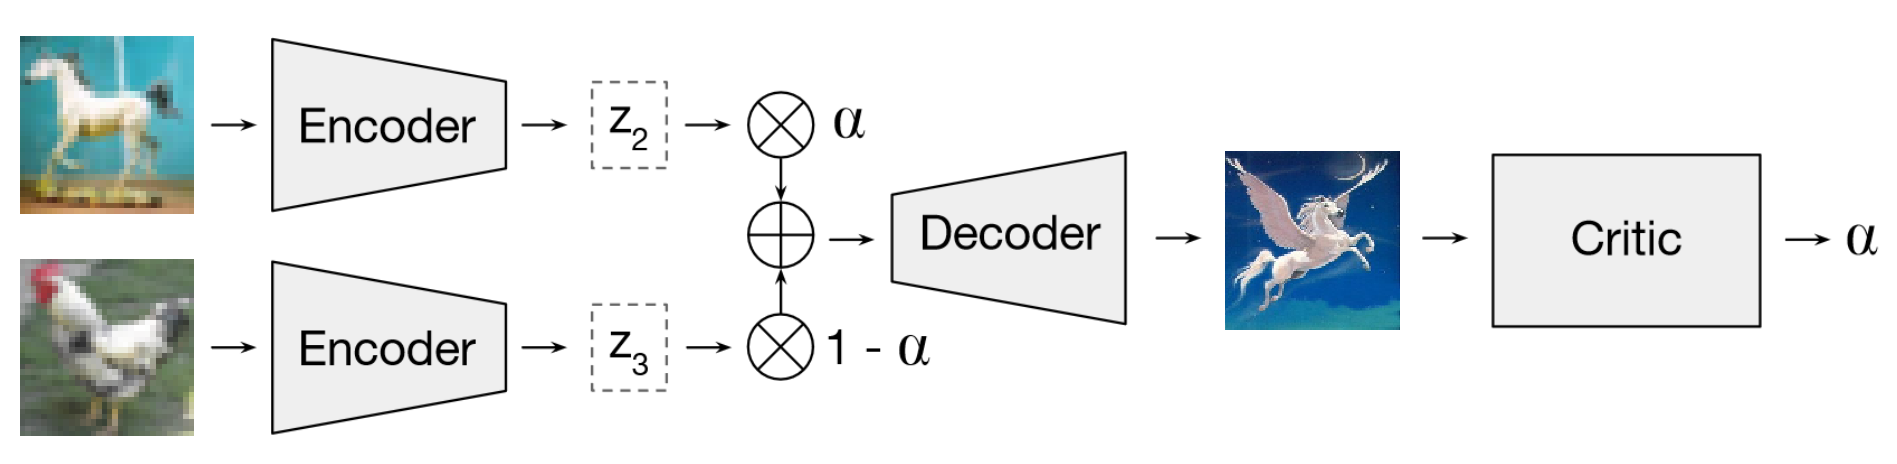
\includegraphics[width=\linewidth]{structure.png}
  \caption{ACAI. A discriminator / critic network is fed interpolants and reconstructions and tries to predict the interpolation coefficient $\alpha$, with $\alpha = 0$ for reconstructions. The autoencoder is trained to fool the critic into outputting $\alpha = 0$ for interpolants.}
\end{figure}

\subsection{Autoencoder}

Autoencoders are typically 'shallow', consisting of only a single-layer encoder and single-layer decoder, but 'deep' autoencoders have been shown to have numerous advantages \cite{goodfellow_et_al_2016} and experimentally yield better compression \cite{hinton_salakhutdinov_2006}. The autoencoder used here is very deep: $18$ layers with the final configuration of hyperparameters.\\

The encoder $f_\theta$ (appendix $3.1$) consists of 'blocks' of two consecutive $3 \times 3$ convolutional layers (\verb|torch.nn.Conv2d|) followed by $2 \times 2$ average pooling (\verb|torch.nn.AvgPool2d|). The number of blocks is computed in such a way to determine the dimension of the latent space. The authors found best results on real-life datasets with a latent space of dimension of $256$ ($16, 4, 4$), which is also used here. After each block is a \verb|LeakyReLU| activation function. Using \verb|LeakyReLU| activation functions with a negative slope of 0.2 appears to be current best practice \cite{berthelot_et_al_2019} \cite{heljakka_solin_kannala_2018}. \verb|tanh| was also tested, but found to offer no improvement.\\

The decoder $g_\phi$ (appendix $3.2$) also consists of 'blocks' of $2 \times 2$ convolutional layers, also with \verb|LeakyReLU|, and followed by $2 \times 2$ nearest neighbour upsampling (\verb|torch.nn.Upsample|). The number of channels is halved after each upsampling layer. After the blocks, two more $3 \times 3$ convolutions are used, with $3$ channels, followed by a final \verb|sigmoid| activation, to convert results to $[0, 1]$ range suitable for display. The use of \verb|torch.nn.ConvTranspose2d| was considered, but current best practice is to use \verb|torch.nn.Upsample| instead to avoid checkboard effects in decoded images.\\ 

Parameters are optimised with Adam \cite{kingma_welling_2014}. The values for the learning rate \verb|l_r = 1e-3| and weight decay \verb|weight_decay = 1e-5| given in \cite{berthelot_et_al_2019} were found to inhibit performance compared to the defaults of \verb|l_r = 1e-5| and \verb|weight_decay = 0|, which are used instead. The authors's custom initialisation of zero-mean Gaussian random variables was discarded. \\

Binary-cross entropy loss (\verb|torch.nn.BCELoss|) was found to offer superior results to the standard mean-squared error (\verb|torch.nn.MSELoss|) used in \cite{berthelot_et_al_2019} so was used instead in conjunction with the original regularisation term.

\subsection{Discriminator}

The discriminator $d_\omega$ uses the same network structure as $f_\theta$. The output of $d_\omega(x)$ is a scalar value, computed as the mean of the encoded input $z = f_\theta(x)$. The discriminator uses spectral normalisation \cite{miyato_2018} to limit variance in discriminator loss, with an over-training ratio controlled by the parameter \verb|disc_train|. Large values ($ >5$) were found to negatively impact the performance of the autoencoder; ultimately, $0$ was used, which likely served to constrain the discriminator.

\subsection{Datasets, samplers, and augmentation}

A custom subclass of \verb|torchvision.datasets.CIFAR10| was used. This comprised $20,000$ images. The first $10,000$ images are horses or deer, the 'body' of the pegasus; the second $10,000$ are birds or planes, the 'wings'. A custom batch sampler was used, such that, in each batch, the first half comprised horses and / or deer, and the second half birds and / or planes.\\

Standard data augmentations were tested.  Random crops and noise were found to decrease the performance of the model. Normalisation is unnecessary when using the built-in transform \verb|torch.transforms.ToTensor|, which converts images to type \verb|torch.FloatTensor|, in the range $[0, 1]$, suitable both for BCE loss functions and sigmoid activation functions. The only augmentation used is a random horizontal flip. 

\subsection{Training}

The model was trained for $250$ epochs, with batches of size $64$, significantly less than the authors' $2^{24}$ samples, but commensurate with available resources. Beyond $250$ losses for both models stopped improving. Training took place on a reasonably powerful machine, with 16GB of RAM, an i5-6660K CPU, and a NVIDA 980GT TI GPU with 8GB of VRAM; each epoch took around $25$s to train. The model uses GPU hardware acceleration by default. 

\begin{figure}[h!]
    \centering
    \subfloat[Autoencoder]{{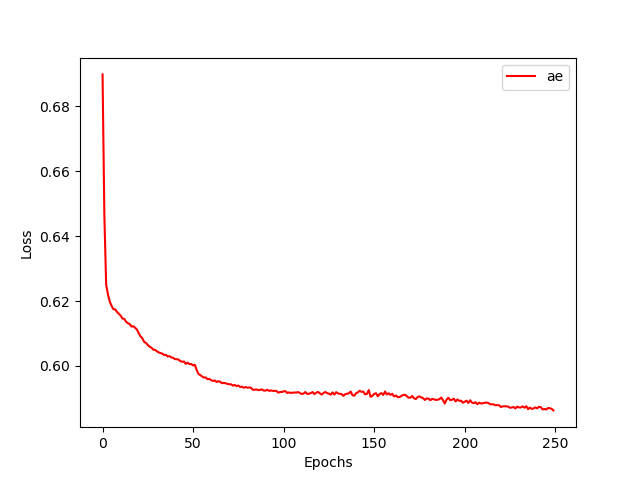
\includegraphics[width=.45\linewidth]{ae.png} }}
    \qquad
    \subfloat[Discriminator]{{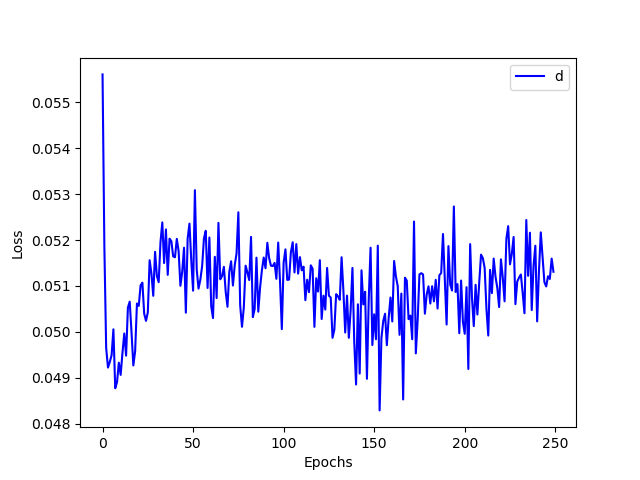
\includegraphics[width=.45\linewidth]{d.png} }}
    \caption{Loss}
\end{figure}

\clearpage
\section{Results}

Results are presented below. They are horse / bird and horse / plane, trained separately.

\begin{figure}[h!]
  \centering
  
\includegraphics{best.png}
  \caption{The best pegasi.}
\end{figure}

\begin{figure}[h!]
  \centering
  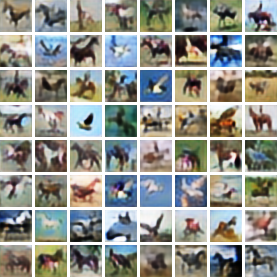
\includegraphics{batch.png}
  \caption{A curated batch of 64 pegasi.}
\end{figure}

\section{Evaluation}

It proved extremely difficult to balance the autoencoder and discriminator. Autoencoder loss would frequently skyrocket as the discriminator reached a tipping point, usually around epoch $20$, at which it considered the problem of predicting $\alpha$ "solved". As generated images are entirely based on discriminator output, this resulted in poor results: images of block colour, in most cases. Attempts to remedy this essentially constrained the performance of the discriminator: removing spectral normalisation, using SGD instead of Adam for optimisation, removing overtraining, and so on. Even with these measures, good results were few and far between. \\

It seems that ACAI is perhaps not the best model for this task. This is believed to be a consequence of the non-convex nature of CIFAR10. MNIST, on which ACAI was first developed, is a very simple dataset. It can be 'solved' using $k$-means clustering. CIFAR10 is very complex. As a result, the latent space manifold is very complex as well. The autoencoder, linearly interpolating between a horse / deer and a bird / plane, likely produces a latent code \textit{outside} the learned space, for which it has little information. Consequently, output images are poor, and the discriminator easily distinguishes between real and reconstructed images. The resulting imbalance produces a convergence in discriminator $\alpha$ predictions, and correspondingly poor pegasi.
\printbibliography

\clearpage
\section{Appendices}

\subsection{Encoder}

\begin{verbatim}

Sequential(
  (0): Conv2d(3, 16, kernel_size=(1, 1), stride=(1, 1), padding=(1, 1))
  (1): Conv2d(16, 16, kernel_size=(3, 3), stride=(1, 1), padding=(1, 1))
  (2): LeakyReLU(negative_slope=0.01)
  (3): Conv2d(16, 16, kernel_size=(3, 3), stride=(1, 1), padding=(1, 1))
  (4): LeakyReLU(negative_slope=0.01)
  (5): AvgPool2d(kernel_size=2, stride=2, padding=0)
  (6): Conv2d(16, 32, kernel_size=(3, 3), stride=(1, 1), padding=(1, 1))
  (7): LeakyReLU(negative_slope=0.01)
  (8): Conv2d(32, 32, kernel_size=(3, 3), stride=(1, 1), padding=(1, 1))
  (9): LeakyReLU(negative_slope=0.01)
  (10): AvgPool2d(kernel_size=2, stride=2, padding=0)
  (11): Conv2d(32, 64, kernel_size=(3, 3), stride=(1, 1), padding=(1, 1))
  (12): LeakyReLU(negative_slope=0.01)
  (13): Conv2d(64, 64, kernel_size=(3, 3), stride=(1, 1), padding=(1, 1))
  (14): LeakyReLU(negative_slope=0.01)
  (15): AvgPool2d(kernel_size=2, stride=2, padding=0)
  (16): Conv2d(64, 128, kernel_size=(3, 3), stride=(1, 1), padding=(1, 1))
  (17): LeakyReLU(negative_slope=0.01)
  (18): Conv2d(128, 16, kernel_size=(3, 3), stride=(1, 1), padding=(1, 1))
)

\end{verbatim}

\clearpage
\subsection{Decoder}

\begin{verbatim}

Sequential(
  (0): Conv2d(16, 64, kernel_size=(3, 3), stride=(1, 1), padding=(1, 1))
  (1): LeakyReLU(negative_slope=0.01)
  (2): Conv2d(64, 64, kernel_size=(3, 3), stride=(1, 1), padding=(1, 1))
  (3): LeakyReLU(negative_slope=0.01)
  (4): Upsample(scale_factor=2.0, mode=nearest)
  (5): Conv2d(64, 32, kernel_size=(3, 3), stride=(1, 1), padding=(1, 1))
  (6): LeakyReLU(negative_slope=0.01)
  (7): Conv2d(32, 32, kernel_size=(3, 3), stride=(1, 1), padding=(1, 1))
  (8): LeakyReLU(negative_slope=0.01)
  (9): Upsample(scale_factor=2.0, mode=nearest)
  (10): Conv2d(32, 16, kernel_size=(3, 3), stride=(1, 1), padding=(1, 1))
  (11): LeakyReLU(negative_slope=0.01)
  (12): Conv2d(16, 16, kernel_size=(3, 3), stride=(1, 1), padding=(1, 1))
  (13): LeakyReLU(negative_slope=0.01)
  (14): Upsample(scale_factor=2.0, mode=nearest)
  (15): Conv2d(16, 16, kernel_size=(3, 3), stride=(1, 1), padding=(1, 1))
  (16): LeakyReLU(negative_slope=0.01)
  (17): Conv2d(16, 3, kernel_size=(3, 3), stride=(1, 1), padding=(1, 1))
  (18): Sigmoid()
)

\end{verbatim}

\end{document}
